\section{Decision Trees}
The space is recursively partitioned, each node in the tree is responsible for establishing a subdivision of the space, the final leaf corresponds to the output.
\begin{itemize}
    \item Each node corresponds to only one attribute
    \item Branching is determined by the value of the attribute
    \item Each leaf is associated with a class
\end{itemize}
For each training set it is possible to general a decision tree with a path to the correct leaf for each sample, the generated tree however does not generalize over other test examples (overfitting). It is therefore necessary to regularize to create more compact trees that can generalize.
\begin{center}
    \begin{tabular}{c c}
        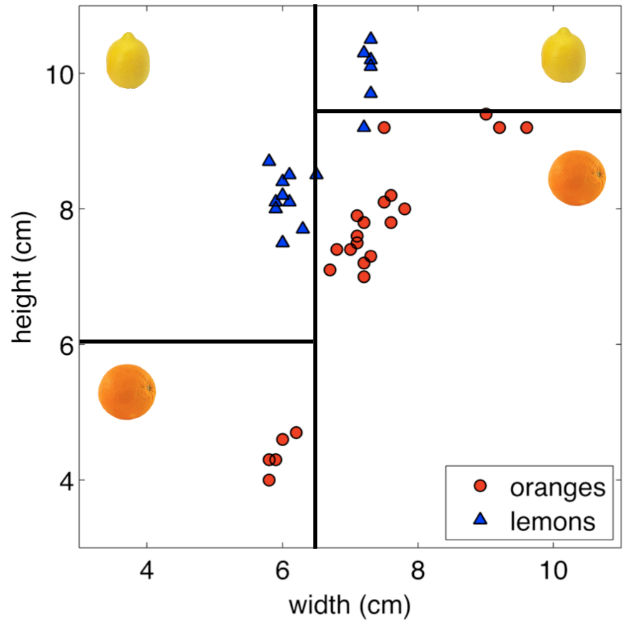
\includegraphics[width=0.45\textwidth]{images/DecisionTrees1.png} &
        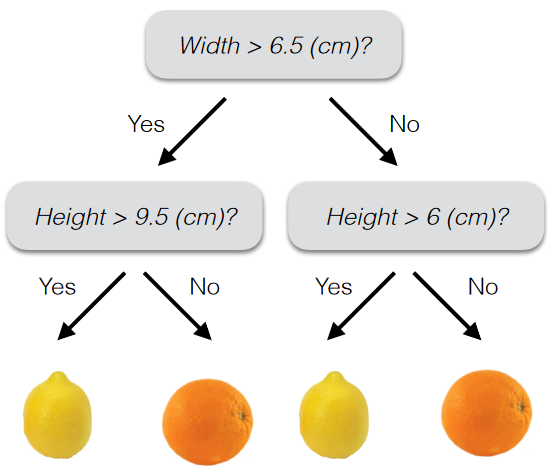
\includegraphics[width=0.5\textwidth]{images/DecisionTrees2.png}
    \end{tabular}
\end{center}

\subsection{Learning Decision Trees}
Creating the simplest decision tree is a complete NP problem, so heuristic solutions are used to simplify the problem:
\begin{enumerate}
    \item start with an empty decision tree
    \item divide the tree on the attribute that subdivides the examples among them in the best way
    \item recursively repeat the process
\end{enumerate}

\subsubsection{ID3 Algorithm}
ID3 is a popular for learning decision trees and works like this:
\begin{enumerate}
    \item creates a root node $r$
    \item if all examples $S$ belong to the same class $y$ returns the root node with label $y$
    \item if $A$ (attributes) is empty it will return $r$ with the same value as the most frequent class in $S$
    \item else select the optimal node:
    \begin{enumerate}
        \item[a.] partitions the set $S$ into subsets using the attribute for which entropy is minimized
        \item[b.] creates a decision node containing the selected attribute
        \item[c.] applies recursion in the underlying branch
    \end{enumerate}
\end{enumerate}

\subsubsection{Entropy}
To choose the optimal attribute, one can use the \textbf{Entropy} $H$, which is the measure of the amount of randomness of a certain dataset $S$, which is defined by the formula:
\begin{equation} \tag{Entropy}
    H(S) = -\sum_{c \in C} p_c\log_2 p_c
\end{equation}
where:
\begin{itemize}
    \item $C$ is the set of all possible classes
    \item $p_c$ is the proportion of elements in $c$ to all elements contained in the dataset $S$
\end{itemize}
\begin{multicols}{2}
    \raggedright % to left align
    In case of \textbf{high entropy} we will have:
    \begin{itemize}
        \item variable with a uniform distribution
        \item flat histogram
        \item less predictable sampled values
    \end{itemize} 
    \columnbreak
    In case of \textbf{low entropy} we will have:
    \begin{itemize}
        \item distribution of the variable with many peaks and valleys
        \item histogram with many highs and lows
        \item more predictable sampled values
    \end{itemize}
\end{multicols}
\begin{mdframed}
    \textbf{Information gain:} entropy-based measure that measures the change in entropy depending on the attribute on which the partitioning is based.
\end{mdframed}
The formula for information gain is as follows:
\begin{equation} \tag{Information gain}
    \text{IG}(S,a) = H(S) - \sum_{t \in T} p_tH_t = H(S) - H(S|a)
\end{equation}
where:
\begin{itemize}
    \item $H(S)$ is the entropy of the dataset $S$
    \item $T$ are the subsets created by splitting $S$ according to the attribute $a$
    \item $p_t$ is the proportion of elements in $t$ to all elements in $S$
    \item $H_t$ is the entropy of the subset $t \in T$
\end{itemize}

\subsection{Characteristics}
What makes a good tree?
\begin{itemize}
    \item Not too small: need to handle important but subtle distinctions in data
    \item Not too large: computational efficiency, avoid overfitting training examples
    \item Occam's Razor: find the simplest hypothesis
    \item Inductive Bias: small trees that place high information gain attributes
    close to the root are preferred
\end{itemize}

\subsection{Issues}
\begin{itemize}
    \item You have exponentially less data at lower levels
    \item Too big of a tree can overfit the data
    \item Greedy algorithms usually don't yield the global optimum
    \item Information gain privileges the attributes that assume a broad range of values
\end{itemize}

\newpage